{\bfseries ҒТАМР 20.15.05}

{\bfseries ЖЕЛІ ҚАУІПСІЗДІГІН ҚАМТАМАСЫЗ ЕТУДЕ ТРАФИКТІ ТАЛДАУ ҚҰРАЛДАРЫН}

{\bfseries ҚОЛДАНУ АРҚЫЛЫ АУЫТҚУЛАР МЕН ЫҚТИМАЛ ҚАУІПТЕРДІ АНЫҚТАУ}

{\bfseries Ж. Бидахмет, А. Уайда, Р.Е.Әлішер, Д. Бағдаулет, Қ. Қаржаубаев
,}

{\bfseries А.Сердалы, Ә. Ахметов}

әл-Фараби атындағы Қазақ ұлттық университеті, Алматы, Қазақстан,

е-mail: uaida\_a@mail.ru

Мақалада компьютерлік желілерде ақпарат жинау әдістері және олардың
қазіргі цифрлық қоғамдағы желілік қауіпсіздікті қамтамасыз етудегі
маңызы қарастырылады, яғни компьютерлік желілердегі ақпаратты түсіру
құралдарының желілік қауіпсіздігі талданады. Қазіргі ақпараттық қоғамда
бұл құралдардың маңызы артып келеді. Трафикті талдау процесі желі арқылы
берілетін деректерді бақылау, жазу және талдау арқылы ауытқулар мен
ықтимал қауіптерді анықтауды қамтиды. Мақалада Wireshark, Tcpdump және
Macof сияқты құралдардың функционалдығы мен қолдану әдістері тереңірек
қарастырылған. Осы құралдарды қолдану әдістері талқыланып, олардың
әрқайсысының ерекшеліктері мен мүмкіндіктері көрсетілген. Әртүрлі
желілік құралдарды тиімді пайдалану арқылы желідегі қауіп-қатерлерді
алдын-ала анықтау және жою мүмкіндігіне баса назар аударылды. Бұл
құралдардың көмегімен желілік қауіпсіздік деңгейін арттыруға, желі
ақауларын жылдам табуға және жоюға болатыны көрсетілген. Сонымен қатар,
мақалада әрбір құралдың артықшылықтары мен кемшіліктерін салыстыра
отырып, олардың қай жағдайда тиімді екені анықталды.

{\bfseries Түйін сөздер:} ақпарат, желі, қауіпсіздік, трафик, Wireshark,
Tcpdump, Macof

{\bfseries ВЫЯВЛЕНИЕ ОТКЛОНЕНИЙ И ПОТЕНЦИАЛЬНЫХ УГРОЗ С ПОМОЩЬЮ
ИНСТРУМЕНТОВ АНАЛИЗА ТРАФИКА В ОБЕСПЕЧЕНИИ}

{\bfseries БЕЗОПАСНОСТИ СЕТИ}

{\bfseries Ж. Бидахмет, А. Уайда, Р.Е. Алишер, Д. Багдаулет, К.
Каржаубаев,}

{\bfseries А.Сердалы, А. Ахметов}

Казахский национальный университет им. Аль-Фараби, Алматы, Казахстан,

е-mail: uaida\_a@mail.ru

В статье рассматриваются методы сбора информации в компьютерных сетях и
их значение для обеспечения сетевой безопасности в современном цифровом
обществе, т. е. анализируется сетевая безопасность средств захвата
информации в компьютерных сетях. В современном информационном обществе
значение этих средств возрастает. Процесс анализа трафика включает
выявление аномалий и потенциальных угроз путем мониторинга, записи и
анализа данных, передаваемых по сети. В статье подробно рассматриваются
функциональные возможности и методы использования таких инструментов,
как Wireshark, Tcpdump и Macof. Обсуждаются методы применения этих
средств, демонстрируются особенности и возможности каждого из них. Упор
был сделан на возможность заранее выявлять и устранять угрозы в сети с
помощью эффективного использования различных сетевых инструментов. Было
показано, что с помощью этих инструментов можно повысить уровень сетевой
безопасности, быстро найти и устранить проблемы с сетью. Кроме того, в
статье сравниваются преимущества и недостатки каждого средства, чтобы
определить, в каких случаях они наиболее эффективны.

{\bfseries Ключевые слова:} информация, сеть, безопасность, трафик,
Wireshark, Tcpdump, Macof

{\bfseries IDENTIFY DEVIATIONS AND POTENTIAL THREATS USING TRAFFIC
ANALYSIS}

{\bfseries TOOLS TO ENSURE NETWORK SECURITY}

{\bfseries Zh.Bidakhmet, A. Uaida, Alisher R., D. Bagdaulet, K.
Karzhaubaev,}

{\bfseries A. Serdaly, A. Akhmetov}

Al-Farabi Kazakh National University, Almaty, Kazakhstan,

е-mail: uaida\_a@mail.ru

The article discusses methods of information capture in computer
networks and their importance for network security in
today\textquotesingle s digital society, i.e. it analyzes the network
security of information capture tools in computer networks. In
today\textquotesingle s information society, the importance of these
tools is increasing. The process of traffic analysis involves
identifying anomalies and potential threats by monitoring, recording and
analyzing data transmitted over the network. The article discusses in
detail the functionality and methods of using tools such as Wireshark,
Tcpdump and Macof. The methods of using these tools are discussed, the
features and capabilities of each of them are demonstrated. The emphasis
was placed on the ability to identify and eliminate threats in the
network in advance through the effective use of various network tools.
It has been shown that using these tools it is possible to increase the
level of network security, quickly find and fix network problems. In
addition, the article compares the advantages and disadvantages of each
remedy to determine in which cases they are most effective.

{\bfseries Keywords:} information, network, security, traffic, Wireshark,
Tcpdump, Macof

{\bfseries Кіріспе.} Қазіргі ақпараттық қоғамда деректерді тасымалдау
әртүрлі желелік орталарда жүзеге асырылады. Сондықтан деректерді
тасымалдау қауіпсіздігін қамтамасыз ету және құпия ақпаратты қорғау
басты мәселе болып табылады. Бұл контексте негізгі аспектілердің бірі
ақпаратты ұстау құралдарын талдау болып табылады.

Деректерді ұстап алу - бұл желі арқылы берілетін немесе электронды түрде
сақталған деректерді заңсыз немесе рұқсат етілген жинау процесі. Бұл
процесс желілік трафикті бақылауды, хабар мазмұнын талдауды және сақтау
құрылғыларынан деректерді жинауды қамтуы мүмкін {[}1{]}.

Желі қауіпсіздігін қамтамасыз етуде трафикті талдау басты рөл атқарады.
Ол желілік инфрақұрылымға бағытталған ықтимал қауіптерді, ауытқуларды
және шабуылдарды анықтауға мүмкіндік береді. Деректердің тасымалдануын
бақылау және пакеттерді талдау арқылы оқиғаларға тез жауап беруге және
құпия ақпараттың ағып кетуіне жол бермеуге болады {[}2{]}.

Трафикті талдау желілік инфрақұрылымның осалдықтарын анықтауға және
жоюға мүмкіндік береді, оның әртүрлі шабуыл түрлерінен сенімді қорғалуын
қамтамасыз етеді. Бұл процесс сонымен қатар желі өнімділігін жақсарту
мүмкіндіктерін анықтау арқылы желі өнімділігін оңтайландыруға
көмектеседі. Тыңдауды талдау желі қауіпсіздігін қамтамасыз ету және
деректердің құпиялылығын қорғаудың маңызды құралы болып табылады.
Төменде біз осы процестің негізгі аспектілерін, трафикті талдау
әдістерін және осы салада тиімді жұмыс істеу үшін қолданылатын
құралдарды қарастырамыз.

{\bfseries Материалдар мен әдістер.} Желілік трафикті талдау құралдары --
компьютерлік желілерде деректердің берілуін бақылауға көмектесетін
бағдарламалар мен утилиталар. Олар желі арқылы өтетін ақпаратты көруге,
талдауға және жазуға мүмкіндік береді. Бұл құралдар желі проблемаларын
анықтауға ғана емес, сонымен қатар деректерді беру қауіпсіздігін
қамтамасыз етуге және желілік трафиктегі ықтимал қауіптер мен
ауытқуларды анықтауға көмектеседі. Бұл мәселелерді тиімді шешу үшін
желілік трафикті талдаудың бірнеше қуатты құралдары бар, олардың
арасында Wireshark, Tcpdump және Macof ерекшеленеді {[}3{]}.

Wireshark -- желі белсенділігін бақылауға, талдауға және жөндеуге
мүмкіндік беретін қуатты желі трафигін талдау құралы. Ол желілік
интерфейс арқылы өтетін деректер пакеттерін ұстап алуға және әрбір пакет
туралы егжей-тегжейлі ақпаратты, соның ішінде протокол тақырыптарын,
деректер мен басқа сипаттамаларды беруге қабілетті.

Wireshark негізгі мүмкіндіктері мен мүмкіндіктеріне мыналар жатады:

\begin{enumerate}
\def\labelenumi{\arabic{enumi}.}
\item
  Қолдау көрсетілетін бірнеше протоколдар: Wireshark 2000-нан астам
  әртүрлі желілік протоколдарды қолдайды, бұл оны әртүрлі желі
  сценарийлерін талдауға арналған әмбебап құрал етеді.
\item
  Графикалық пайдаланушы интерфейсі (GUI): Қарапайым және интуитивті
  интерфейс Wireshark-пен жұмыс істеуді тәжірибелі және жаңадан бастаған
  пайдаланушылар үшін ыңғайлы етеді.
\item
  Сүзу және іздеу: үлкен көлемдегі деректерді өңдеуді жеңілдете отырып,
  тек қажетті ақпаратты бөлектеуге және талдауға мүмкіндік береді.
\end{enumerate}

Wireshark - желі әкімшілері, қауіпсіздік инженерлері, желілік
қосымшаларды әзірлеушілер және желілік инфрақұрылыммен жұмыс істейтін
кез келген басқа адамдар үшін маңызды құрал.

Tcpdump -- желілік трафикті талдауға арналған пәрмен жолы утилитасы. Ол
компьютердің желілік интерфейсі арқылы өтетін деректер пакеттерін
ұстауға және көрсетуге мүмкіндік береді. Tcpdump бағдарламасының маңызды
ерекшелігі оның нақты уақыт режимінде жұмыс істеу мүмкіндігі болып
табылады, бұл оны желі мәселелерін диагностикалау және талдау үшін
қуатты құрал етеді {[}4{]}.

Tcpdump негізгі мүмкіндіктері мен функцияларына мыналар жатады:

\begin{enumerate}
\def\labelenumi{\arabic{enumi}.}
\item
  Көп протоколды қолдау: Tcpdump TCP, UDP, ICMP және т.б. сияқты әртүрлі
  желілік протоколдарды пайдаланып пакеттерді талдауға қабілетті.
\item
  Трафикті сүзу: пайдаланушыға тек белгілі бір пакеттерді (мысалы,
  дереккөз, тағайындалған орын, порт және басқа параметрлер бойынша)
  көрсету үшін нақты критерийлерді көрсетуге мүмкіндік береді.
\item
  Файлдарды оқу және жазуды қолдау: Tcpdump желі трафигінің сақталған
  файлдарымен жұмыс істей алады, сонымен қатар кейінірек талдау үшін
  файлға ағымдағы трафикті жаза алады.
\end{enumerate}

Tcpdump -- желі әкімшілері, қауіпсіздік инженерлері және желілік
трафикті талдаумен жұмыс істейтін кез келген адам үшін маңызды құрал.

Macof - бұл кездейсоқ MAC мекенжайларының үлкен санын жасауға және
оларды желіге жіберуге арналған пәрмен жолы құралы. Macof
бағдарламасының негізгі мақсаты - желі жұмысын баяулату немесе бұзу үшін
жалған MAC мекенжайларының көп санын жасау {[}5{]}.

Macof көмегімен жалған MAC мекенжайларын жасау мүмкіндіктері мыналарды
қамтиды:

\begin{enumerate}
\def\labelenumi{\arabic{enumi}.}
\item
  Кездейсоқ генерация: Macof MAC мекенжайларын кездейсоқ түрде жасайды,
  бұл оларды болжауды қиындатады.
\item
  Желіге жіберу: Жасалған MAC мекенжайлары компьютердің желілік
  интерфейсі арқылы желіге жіберіледі.
\item
  Ықтимал шабуылдар: Macof коммутаторлар сияқты желілік құрылғыларды
  шамадан тыс жүктеуге немесе баяулатуға бағытталған шабуылдарда
  қолданылуы мүмкін.
\end{enumerate}

Macof пайдалану сақтықты қажет ететінін ескеру маңызды, себебі бұл
құралды дұрыс пайдаланбау желінің бұзылуына және қажетсіз жүктемеге
әкелуі мүмкін. Ол көбінесе желілік қауіпсіздікті тестілеуде және желіні
оқытуда қолданылады.

{\bfseries Нәтижелер мен талқылау.} Wireshark мысалы: Енді біз Wireshark
трафикті ұстау және талдау мүмкіндіктерін көрсетеміз. Wireshark-ты іске
қосып, тізімнен бақылау интерфейсін таңдайық, біздің жағдайда бұл eth0
болады (1-сурет).

Интерфейсті таңдағаннан кейін деректерді жинау басталады. Тараудың
басында біз сымсыз желілердегі трафикті бақылау өте қарапайым екенін
айттық. Міне осылай - сымсыз желідегі барлық компьютерлерден деректерді
көру үшін сізге қажетті интерфейсті таңдау керек.

\begin{longtable}[]{@{}
  >{\raggedright\arraybackslash}p{(\columnwidth - 2\tabcolsep) * \real{0.4984}}
  >{\raggedright\arraybackslash}p{(\columnwidth - 2\tabcolsep) * \real{0.5016}}@{}}
\toprule\noalign{}
\begin{minipage}[b]{\linewidth}\raggedright
% \begin{figure}[H]
% 	\centering
% 	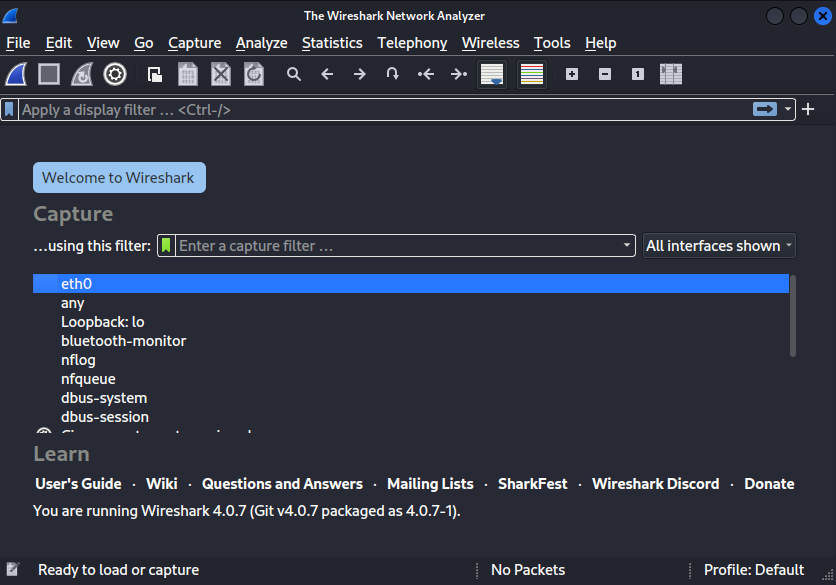
\includegraphics[width=0.8\textwidth]{assets/26}
% 	\caption*{}
% \end{figure}

{\bfseries 1-сурет - Интерфейсті таңдау}
\end{minipage} & \begin{minipage}[b]{\linewidth}\raggedright
% \begin{figure}[H]
% 	\centering
% 	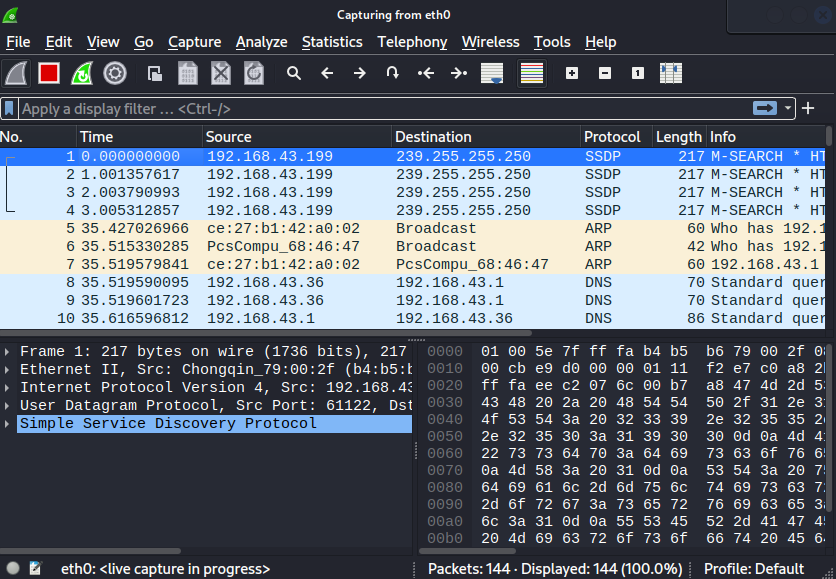
\includegraphics[width=0.8\textwidth]{assets/27}
% 	\caption*{}
% \end{figure}

{\bfseries 2-сурет -Жиналған пакеттер}
\end{minipage} \\
\midrule\noalign{}
\endhead
\bottomrule\noalign{}
\endlastfoot
\end{longtable}

Қажетті деректер көлемін жинағаннан кейін пакеттерді жинауды тоқтатыңыз
(2-сурет). Енді оларды кейінірек талдау үшін сақтауға немесе оны бірден
бастауға болады. Бірнеше минут ішінде біз 20 000-ға жуық пакет жинадық,
бұл желідегі трафик аз болған жағдайда болды. Әрине, мұндай пакеттерді
қолмен қарау өте көп еңбекті қажет ететін жұмыс және оны жеңілдету үшін
Wireshark әртүрлі сүзгілерді ұсынады (1-кесте).

{\bfseries 1-кесте - Wireshark сүзгілері}

\begin{longtable}[]{@{}
  >{\raggedright\arraybackslash}p{(\columnwidth - 4\tabcolsep) * \real{0.3333}}
  >{\raggedright\arraybackslash}p{(\columnwidth - 4\tabcolsep) * \real{0.3333}}
  >{\raggedright\arraybackslash}p{(\columnwidth - 4\tabcolsep) * \real{0.3334}}@{}}
\toprule\noalign{}
\begin{minipage}[b]{\linewidth}\raggedright
Оператор
\end{minipage} & \begin{minipage}[b]{\linewidth}\raggedright
Функция
\end{minipage} & \begin{minipage}[b]{\linewidth}\raggedright
Мысал
\end{minipage} \\
\midrule\noalign{}
\endhead
\bottomrule\noalign{}
\endlastfoot
== & Тең & Ip.addr == 192.168.10.12 \\
eq & Тең & Tcp.port eq 80 \\
!= & Тең емес & Ip.addr != 192.168.10.5 \\
ne & Тең емес & Ip.src ne 192.168.10.5 \\
contains & Құрамында & Hhtp contains ``google.com'' \\
\end{longtable}

Google.com веб-сайтына пайдаланушы сұрауларын сүзгіден өткізейік. DNS
сұрауынан бастайық, өйткені ол әрқашан бірінші болады. Сүзгіні қолдану
арқылы біз браузер сұрауларының және DNS серверіне жауаптардың толық,
дәйекті тарихын көреміз. Енді қай IP мекенжайы әрі қарай байланыс
болатынын біле отырып, сәйкес сүзгіні жасайық (ip.addr==192.168.43.36)
(3-сурет).

\begin{figure}[H]
	\centering
	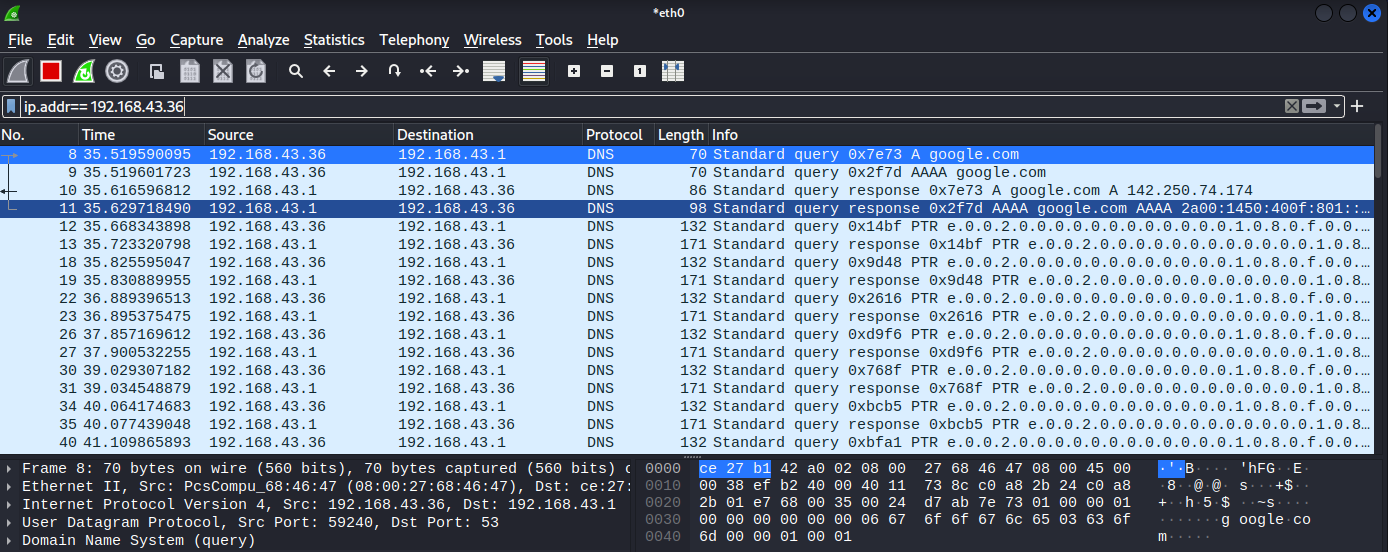
\includegraphics[width=0.8\textwidth]{assets/28}
	\caption*{}
\end{figure}

{\bfseries 3-сурет- Веб-сервермен байланыс}

Көріп отырғаныңыздай, сүзгіден өткен пакеттердің саны 1153 (3-сурет).
Олардың әрқайсысы деректердің аз ғана бөлігін ғана жібереді және оларда
қандай ақпарат бар екенін түсіну өте қиын. Тапсырманы жеңілдету үшін
Wireshark нақты деректер ағынын бақылаудың керемет мүмкіндігіне ие. UDP
жағдайында «UDP Stream» опциясын таңдаңыз {[}6{]}.

Сонымен, біз байланыстың толық, стандартты бейнесін көрдік - DNS
серверінен сұраныс пен жауап, үш жақты қол алысу және деректерді беруді
инициализациялау. Оның үстіне біз пакеттердің мазмұнын да көрдік
(5-сурет).

\begin{figure}[H]
	\centering
	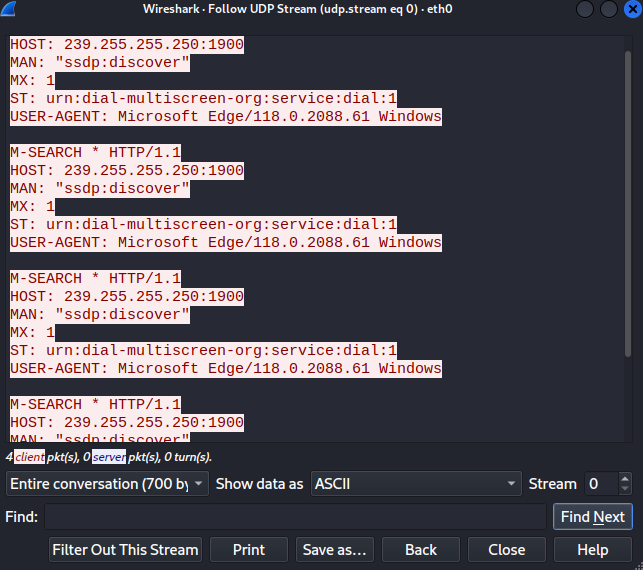
\includegraphics[width=0.8\textwidth]{assets/29}
	\caption*{}
\end{figure}

{\bfseries 5-сурет- Барлық пайдалы ақпарат бір жерде}

Графикалық интерфейске әрқашан қол жеткізе алмайтыныңызды ескеріңіз,
сондықтан Wireshark алдында пайда болған басқа құрал - tcpdump-пен
танысуды ұсынамыз.

Tcpdump мысалы: Егер сіз жай ғана tcpdump іске қоссаңыз, онда барлық
ақпарат нақты уақыт режимінде шығарылады, бұл кейіннен оны талдау үшін
іс жүзінде жарамсыз етеді (6-сурет).

\begin{figure}[H]
	\centering
	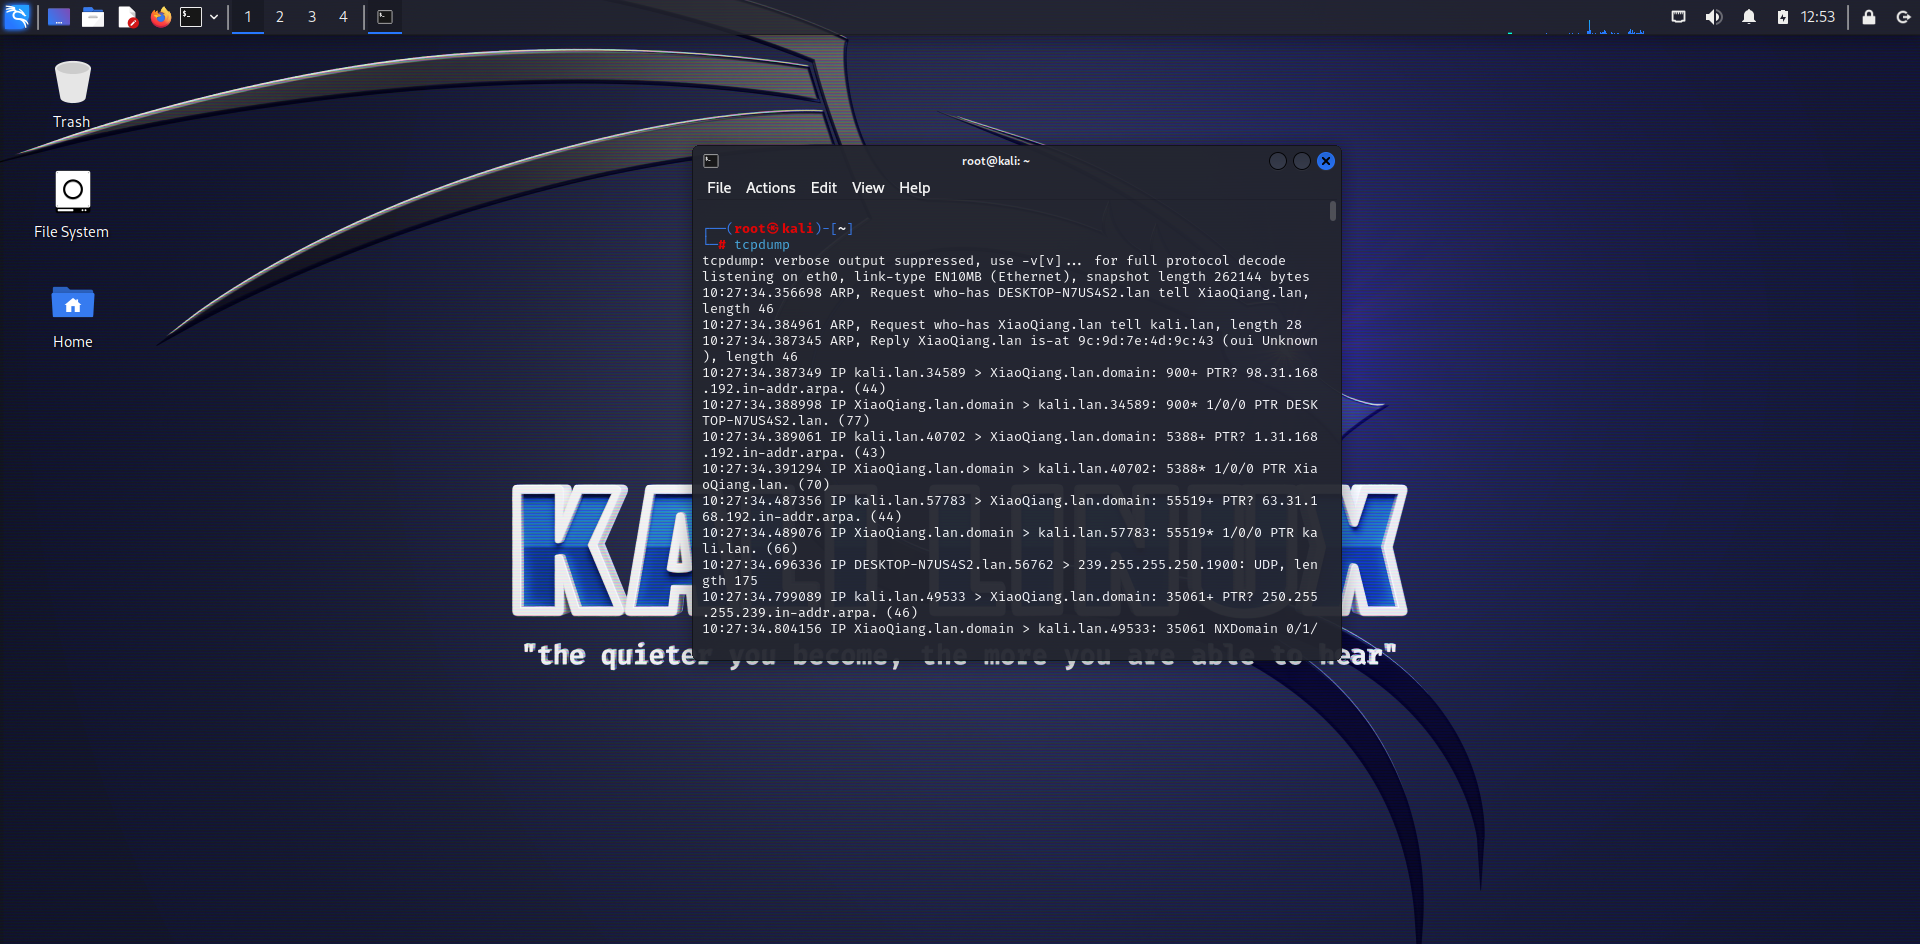
\includegraphics[width=0.8\textwidth]{assets/30}
	\caption*{}
\end{figure}

{\bfseries 6-сурет -Tcpdump командасының нәтижесі}

Барлық ақпаратты файлға сақтау әлдеқайда жақсы, өйткені бұл деректерді
жинауды жеңілдетеді және сізге ыңғайлы кез келген уақытта кейінгі
трафикті талдау мүмкіндігін жасайды (7-сурет).

\begin{figure}[H]
	\centering
	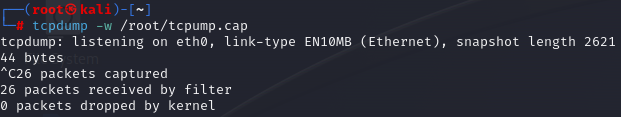
\includegraphics[width=0.8\textwidth]{assets/31}
	\caption*{}
\end{figure}

{\bfseries 7-сурет- Ақпаратты tcpump.cap парақшасына сақтаймыз}

Алынған деректерді талдау үшін консольді пайдалануға болады. Біз дәйекті
боламыз және консольдегі деректерді талдауға мысал келтіреміз.

Қосылым болған барлық IP мекенжайлары мен порттарын қарастырайық
(8-сурет):

\begin{figure}[H]
	\centering
	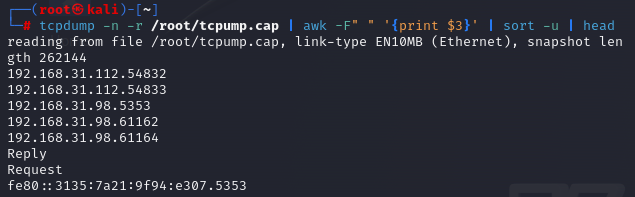
\includegraphics[width=0.8\textwidth]{assets/32}
	\caption*{}
\end{figure}

{\bfseries 8-сурет- Қосылған IP мекенжайлар тізімі}

Әрі қарай, оны түсіру кезінде желі арқылы жіберілген ақпаратты
қарастырайық. Бұл жағдайда біз оны HEX форматында көреміз, бірақ бұл
бізге қажетті деректерді алуға кедергі болмайды (9-сурет).

\begin{figure}[H]
	\centering
	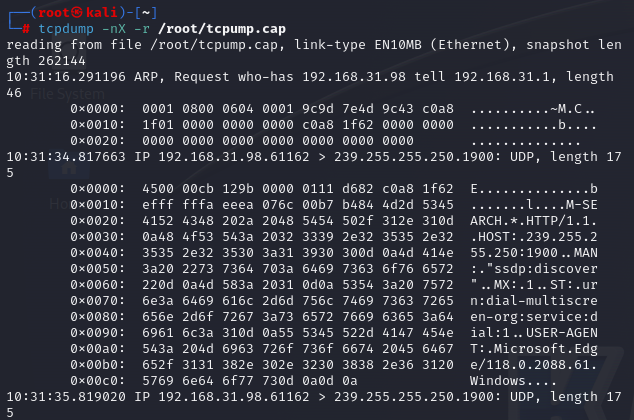
\includegraphics[width=0.8\textwidth]{assets/33}
	\caption*{}
\end{figure}

{\bfseries 9-сурет -Жіберілген ақпараттар HEX-форматында}

Енді шабуылдаушы коммутатор порттарының біріне қол жеткізе алатын
жағдайды қарастырайық. Бұл жағдайда коммутатордың өзіне қол жеткізу
немесе оның басқа бөлмеде орналасқан желілік жабдыққа қосылған желілік
розетка екендігі маңызды емес. Жалғыз маңызды нәрсе - желілік интерфейс
тек келуі керек пакеттерді қабылдайды, одан артық емес.

Мұндай қорғанысты айналып өтудің және коммутаторды хаб ретінде жұмыс
істеуге мәжбүрлеудің ең танымал тәсілдерінің бірі, бұл бізге барлық
желілік трафикті тоқтатуға мүмкіндік береді, CAM кестесін толтыру болып
табылады {[}7-8{]}.

CAM кестесін MAC мекенжайларымен толтыруға бағытталған шабуылды орындау
үшін бір пәрмен жеткілікті (10-сурет):

\begin{figure}[H]
	\centering
	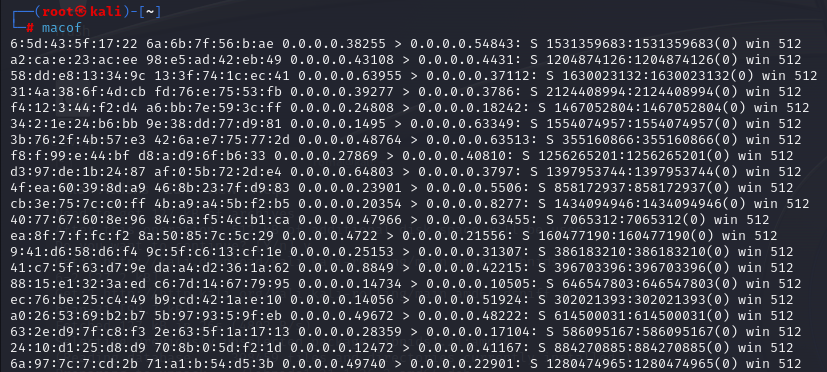
\includegraphics[width=0.8\textwidth]{assets/34}
	\caption*{}
\end{figure}

{\bfseries 10-сурет - Macof шабуылы}

Тағы бір айта кететін мәселе бар. Егер сіз желілік порттардың біріне қол
жеткізсеңіз де, сіз әлі де желіге кіре алмайсыз, өйткені барлық заманауи
коммутаторлар MAC мекенжайлары бойынша қол жеткізуді басқара алады.
Дегенмен, сізде әрқашан компьютердің MAC мекенжайын келесідей өзгерту
мүмкіндігі бар (11-сурет):

\begin{figure}[H]
	\centering
	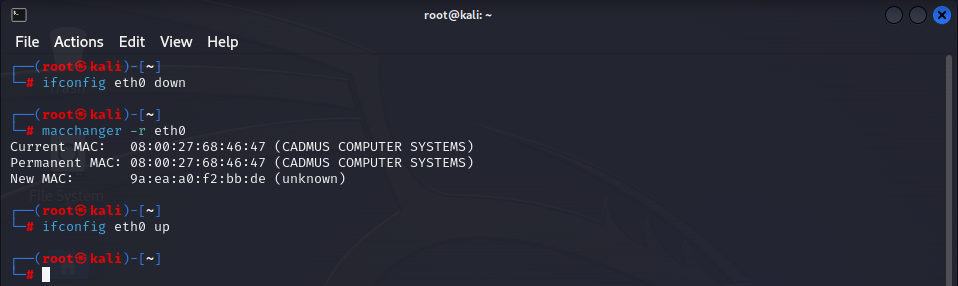
\includegraphics[width=0.8\textwidth]{assets/35}
	\caption*{}
\end{figure}

{\bfseries 11-сурет- MAC мекенжайына өзгертулер}

Трафик талдауы желі өнімділігі туралы құнды түсінік береді және
қауіпсіздік үшін маңызды болуы мүмкін. Дегенмен, оны өткізу кезінде
этикалық нормаларды сақтауды ұмытпаған жөн. Пайдаланушы деректерінің
құпиялылығы мен құпиялылығын ескеру қажет. Жол қозғалысын талдау
нәтижесінде алынған ақпаратты жинау, талдау және сақтау кезінде
деректерді қорғаудың барлық заңдары мен саясаттарын сақтау ұсынылады.

Деректерді қорғаудың криптографиялық әдістерінің дамуымен шифрланған
трафикті талдау барған сайын қиындай түсуде. Шифрлау пакет мазмұнын
егжей-тегжейлі талдауға елеулі кедергі келтіруі мүмкін. Сарапшылар
шифрланған трафикпен жұмыс істеу дағдыларын дамытуы және шифрланған
байланыстағы қауіптерді анықтай және талдай алатын талдау әдістерін
іздеуі керек {[}9{]}.

Бұл аспектілер трафикті талдаумен жұмыс істеу кезінде аналитиктер
кездесетін шектеулер мен қиындықтарды түсіну үшін маңызды. Осы
факторларды ескере отырып, сарапшылар анағұрлым тиімді талдау
стратегиялары мен әдістерін жасай алады. Технологияның дамуымен және
желілік трафиктің жаңа түрлерінің пайда болуымен оны талдаудың
инновациялық тәсілдерінің қажеттілігі туралы сұрақ туындайды. Желінің
қауіпсіздігі және трафикті талдау саласындағы жетекші сарапшылар
қауіптерді тиімдірек анықтап, талдай алатын жаңа әдістер мен
алгоритмдерді құрумен айналысуда. Трафикті талдау саласында жасанды
интеллект, машиналық оқыту және үлкен деректерді талдауды пайдалану
перспективалы бағыт болып табылады {[}10{]}.

Басқа қауіпсіздік құралдарымен интеграция. Желінің тиімді қауіпсіздігі
кешенді тәсілді қажет етеді. Трафикті талдауды басқа қауіпсіздік
құралдарымен, мысалы, қауіпті бақылау жүйелерімен, шабуылды анықтау
құралдарымен және DDoS қорғау жүйелерімен біріктіру желілік
инфрақұрылымды қорғаудың сенімді және тиімді тетіктерін жасауға
мүмкіндік береді {[}11{]}.

{\bfseries Қорытынды.} Зерттеуде желілік трафикті талдаудың негізгі
аспектілері, соның ішінде қолданылатын құралдар, талдау әдістері,
сондай-ақ осы саланың дамуындағы шектеулер мен перспективалар
қарастырылды. Wireshark, Tcpdump және Macof сияқты маңызды құралдардың
мүмкіндіктері мен қолданбалары талқыланды. Желілік трафикті талдаудың
әртүрлі аспектілері, соның ішінде аномалияларды анықтау, желі
өнімділігін бақылау және қауіпсіздік инциденттерін зерттеу әдістері
қарастырылды.

Желілік трафикті талдау құралдарын пайдалану желі қауіпсіздігін
қамтамасыз етудің маңызды элементі болып табылады. Бұл құралдар
аномалияларды анықтап, қауіптерді тауып, желінің жағдайын бақылап,
қауіпсіздік инциденттеріне жауап беруге мүмкіндік береді. Трафикті
талдау арқылы мамандар қауіптерге жылдам жауап беріп, шабуылдардың алдын
алып, желілік инфрақұрылымның үздіксіз жұмысын қамтамасыз етеді.

Желілік трафикті талдау құралдарын пайдалану желінің қауіпсіздік
деңгейін айтарлықтай арттырып, өзгермелі жағдайлар мен қауіптерге жылдам
әрекет етуге мүмкіндік береді. Трафикті талдаудың заманауи әдістерін
әзірлеу және енгізу, оны басқа қауіпсіздік құралдарымен біріктіру және
осы саладағы өзгерістерді үздіксіз бақылау желілік инфрақұрылымның
қауіпсіздігін қамтамасыз етудегі маңызды қадамдар болып табылады.

{\bfseries Әдебиеттер}

1.Chris Sanders~Practical Packet Analysis, 3rd Edition: Using Wireshark
to Solve Real-World Network Problems~3rd Edition// No Starch Press.
-2017.- P.120-145, 2017. ISBN: 978-1593278021

2. Chris Sanders,~Jason Smith~ Applied Network Security Monitoring:
Collection, Detection, and Analysis~1st Edition// Syngress.-2013.-
P.200-210. ISBN 978-0124172081.

3.Michael Sikorski,~Andrew Honig~Practical Malware Analysis: The
Hands-On Guide to Dissecting Malicious Software~1st Edition// No Starch
Press.-2012.-P.325. ISBN: 978-1593272906

4. Sherri Davidoff,~Jonathan Ham Network Forensics: Tracking Hackers
through Cyberspace~1st Edition.//Prentice Hall. -2012.-576 P. ISBN
978-0132564717

5. Laura Chappell Wireshark Network Analysis (Second Edition): The
Official Wireshark Certified Network Analyst Study Guide~2nd Revised ed.
Edition// University Laura Chappell.-2012.- P.250-256. ISBN
978-1893939943

6. Richard Stevens TCP/IP Illustrated: The Protocols, Volume 1
(Addison-Wesley Professional Computing Series)~2nd Edition.-2011.-P.
65-75. ISBN: 978-0321336316.

7. William Stallings~Network Security Essentials: Applications and
Standards~6th Edition.-2016.- P.290-302.ISBN: 978-0134527338

8.A. Rahmatulloh, R. Gunawan, and F. M. S. Nursuwars Performance
comparison of signed algorithms on JSON Web Token //in IOP Conference
Series: Materials Science and Engineering.- 2019.- Vol.550(1):012023.
DOI 10.1088/1757-899X/550/1/012023

9. A. Neumann, N. Laranjeiro, J. Bernardino An Analysis of Public REST
Web Service APIs //IEEE Trans Serv Comput.- 2021.- Vol. 14(4).-
P.957-970. DOI 10.1109/TSC.2018.2847344.

10. G. Alonso, F. Casati, H. Kuno, V. Machiraju. Web Services// in Web
Services: Concepts, Architectures and Applications- Eds. Berlin,
Heidelberg: Springer Berlin Heidelberg.- 2004.- P. 123-149. DOI
10.1007/978-3-662-10876-5\_5.

11.\hl{Бидахмет Ж.,Уайда А., Майлыбаева А.Д., Даркенбаев Д.К.,Бекназаров
С.,Бағдаулет Д. Metasploit framework арқылы желі мен сервердегі
осалдықтарды сканерлеу және операциялық жүйелерге қашықтан қол жеткізу.-
Вестник КазУТБ.-2024- № 1(22).- С.97-106}

\emph{{\bfseries Авторлар туралы мәліметтер}}

Бидахмет Ж. - PhD, әл-Фараби атындағы Қазақ ұлттық университетінің м.а.
доценті, Алматы, Қазақстан,e-mail:bidakhmetzhanar@gmail.com;

Уайда А. -- әл-Фараби атындағы Қазақ ұлттық университетінің магистранты,
Алматы, Қазақстан, e-mail: uaida\_a@mail.ru;

Бағдаулет Д. - әл-Фараби атындағы Қазақ ұлттық университетінің
магистранты, Алматы, Қазақстан, e-mail: dasik-007@mail.ru;

Әлішер Р. - әл-Фараби атындағы Қазақ ұлттық университетінің магистранты,
Алматы, Қазақстан, e-mail: roma43529@gmail.com;

Қаржаубаев Қ. - әл-Фараби атындағы Қазақ ұлттық университетінің
магистранты, Алматы, Қазақстан, e-mail: Karzhaubayevkuanysh@gmail.com;

Сердалы А.- әл-Фараби атындағы Қазақ ұлттық университетінің магистранты,
Алматы, Қазақстан, e-mail: altynayserdaly@gmail.com;

Ахметов Ә. - әл-Фараби атындағы Қазақ ұлттық университетінің
магистранты, e-mail: Aahmetov755@gmail.com;

\emph{{\bfseries Information about authors}}

Bidakhmet Zh.- PhD,Acting Associate Professor NAO Al-Farabi Kazakh
National University, Almaty, Kazakhstan, e-mail:
bidakhmetzhanar@gmail.com;

Uaida A. - graduate student at Al-Farabi Kazakh National University,
Almaty, Kazakhstan, e-mail: uaida\_a@mail.ru;

Bagdaulet D. - graduate student at Al-Farabi Kazakh National University,
Almaty, Kazakhstan, e-mail: dasik-007@mail.ru;

Alisher R. -graduate student of Al-Farabi Kazakh National University,
Almaty, Kazakhstan,e-mail: roma43529@gmail.com;

Karzhaubaev K.- graduate student of Al-Farabi Kazakh National
University, Almaty, Kazakhstan, e-mail: Karzhaubayevkuanysh@gmail.com;

Serdaly A.-graduate student of Al-Farabi Kazakh National University,
Almaty, Kazakhstan, e-mail: altynayserdaly@gmail.com;

Akhmetov A.-graduate student of Al-Farabi Kazakh National University,
Almaty, Kazakhstan,

e-mail:Aahmetov755@gmail.com
